\documentclass[11pt]{article}
\usepackage[top=1in, bottom=1.25in, left=1.25in, right=1.25in]{geometry}
\newcommand{\tabitem}{~~\llap{\textbullet}~~}
\usepackage[parfill]{parskip}
\usepackage{enumerate,amsmath,amsthm,amssymb,bbold}
\usepackage{minibox,graphicx,caption,booktabs,pdflscape,multirow,verbatim,subcaption,pdfpages,longtable}
\usepackage[shortlabels]{enumitem}
\usepackage[T1]{fontenc}
\usepackage[section]{placeins} %to keep graphs and tables in the very section to which they belong 
%-----------------------------------------------------------------------------
\begin{document}
\begin{center}
\framebox[\linewidth]{ 
	\minibox[c]{
	\Large Homework \#2 \\ \\
	Professor: Pat Kline \\ \\
	Students: Christina Brown, Sam Leone, Peter McCrory, Preston Mui
	}
}
\end{center}

\subsection*{2. Logit MLE}

\begin{enumerate}[a)]

	\item Derive the score of the logit-likelihood:
	First, noting that
	\begin{align*}
		\frac{\partial \Lambda(X_i'\beta)}{\partial \beta} &= \frac{\exp(X_i' \beta)X_i'(1 + X_i'\beta) - \exp(X_i'\beta) \exp(X_i'\beta) X_i'}{(1+\exp(X_i'\beta))^2} = \frac{\exp(X_i'\beta)X_i'}{(1 + \exp(X_i'\beta))^2}
	\end{align*}
	The score of the logit log-likelihood is therefore
	\begin{align*}
		s(\beta) &= \sum_i \frac{Y_i \exp(X_i'\beta)X_i' }{\Lambda(X_i'\beta)(1 + \exp(X_i'\beta))^2} -
			\frac{(1 - Y_i)\exp(X_i'\beta)X_i'}{(1 - \Lambda(X_i'\beta))(1 + \exp(X_i'\beta))^2} \\
		&= \sum_i \Big( Y_i - (1 - Y_i)\exp(X_i'\beta) \Big) \frac{X_i'}{1 + \exp(X_i'\beta)}\\
		&= \sum_i \Big( Y_i(1 + \exp(X_i'\beta)) - \exp(X_i'\beta) \Big) \frac{X_i'}{1 + \exp(X_i'\beta)} \\
		&= \sum_i \Big( Y_i - \frac{\exp(X_i'\beta)}{1 + \exp(X_i'\beta)} \Big) X_i'
	\end{align*}
	
	\item The moment condition identifying $\beta_{ML}$ is
	\begin{align*}
		E \bigg[ \Big( Y_i - \frac{\exp(X_i'\beta)}{1 + \exp(X_i'\beta)}\Big) X_i' \bigg] &= 0 \\
		E \bigg[ E[Y_i - \frac{\exp(X_i'\beta)}{1 + \exp(X_i'\beta)} | X_i] X_i' \bigg] &= 0
	\end{align*}
	
	\item The moment conditions identifying $\beta_{NLLS}$ are
	\begin{align*}
		0 &= E \bigg[ -2 (Y_i - \Lambda(X_i'\beta)) \frac{\exp(X_i'\beta)}{(1 + \exp(X_i'\beta))^2} X_i' \bigg] \\
		&= E \bigg[ E[(Y - \Lambda(X_i'\beta)) | X_i] \frac{\exp(X_i'\beta)}{(1 + \exp(X_i'\beta))^2} X_i' \bigg] \\
	\end{align*}

	\item Under which conditions does $\beta_{NLLS}$ coincide with $\beta_{ML}$? The moment conditions will coincide when $E[Y_i - \Lambda(X_i'\beta) | X_i'] = 0$ for all $X_i$; that is, they coincide when the logit model is correctly specified.

\end{enumerate}


\subsection*{3. Matlab Probit DGP}

\begin{enumerate}[a)]

	\item (Matlab program attached)

	\item The ML point estimates of $\hat{\beta}^{con} = (\hat{\alpha},\hat{b})$ are $(-0.0175,0.9159)$. The standard errors are $(0.3030,0.3607)$, respectively.

	\item Score test: Following Wooldridge (2010), page 570, the $LM$ statistic is the ESS from the following regression
	\begin{align*}
		\frac{\hat{u}_i}{\sqrt{\hat{G}_i (1 - \hat{G}_i)}} &= \alpha \frac{\hat{g}_i}{\sqrt{\hat{G}_i(1 - \hat{G}_i)}} x_i + \gamma  \frac{\hat{g}_i}{\sqrt{\hat{G}_i(1 - \hat{G}_i)}} z_i
	\end{align*}
	where $x_i$ is the regressor matrix in the unconstrained regression (constant and $X$) and $z_i$ is the vector of $X_i^2$. The ESS from this regression was $0.2963$, which has a p-value of $0.58621$. So, one does not reject the null that $b_2 = 0$.

	\item The unrestricted model yields point estimates of $\hat{\beta}^{unc} = (\hat{\alpha},\hat{b},\hat{b_2}) = (-0.0435, 0.9175, 0.0428)$. The Wald test will test the null $g(\beta) = 0$ where
	\begin{align*}
		g(\beta) &\equiv (0, 0, 1) \cdot \beta = b_2 \\
		G(\beta) &\equiv \frac{\partial g(\beta)}{\partial \beta} = (0, 0, 1)
	\end{align*}
	and the Wald statistic is given by
	\begin{align*}
		N \cdot \hat{b_2} \cdot \bigg( G \cdot \frac{1}{\sqrt{N}}H^{-1} \cdot G' \bigg)^{-1} \cdot \hat{b_2}
	\end{align*}
	where $H$ is the average Hessian at the ML estimate. Because we know that the model is correctly specified, I use the inverse Hessian instead of the sandwich estimator. The Wald evaluates to 7.4592, which has a p-value of $0.0063$ under the $\chi^2$ distribution with d.f. 1, so one rejects the null that $b_2 = 0$. This is starkly different from the score test result, which did not reject the null. This makes sense, as the Wald tends to reject more than the LM test. If one bumps the number of observations up (say, to 5000), both tests reject the null.

\end{enumerate}

\subsection*{4. Clustered DGP in Stata}

\begin{enumerate}[a)]

	\item Regressing $Y_{ic}$ on $D_{ic}$, we get the results in table 1.
		\begin{table}[htbp]\centering
\def\sym#1{\ifmmode^{#1}\else\(^{#1}\)\fi}
\caption{Clustered DGP}
\begin{tabular}{l*{3}{c}}
\toprule
                    &\multicolumn{1}{c}{(1)}&\multicolumn{1}{c}{(2)}&\multicolumn{1}{c}{(3)}\\
                    &\multicolumn{1}{c}{Y\_ic, Regular SE}&\multicolumn{1}{c}{Y\_ic, Robust SE}&\multicolumn{1}{c}{Y\_ic, Clustered SE}\\
\midrule
d\_ic                &       1.010***&       1.010***&       1.010***\\
                    &   (0.03237)   &   (0.03244)   &   (0.09508)   \\
\addlinespace
Constant            &      0.0394*  &      0.0394*  &      0.0394   \\
                    &   (0.02278)   &   (0.02037)   &   (0.10761)   \\
\midrule
\(R^{2}\)           &       0.089   &       0.089   &       0.089   \\
Observations        &       10000   &       10000   &       10000   \\
\bottomrule
\multicolumn{4}{l}{\footnotesize Standard errors in parentheses}\\
\multicolumn{4}{l}{\footnotesize * p<0.10, ** p<0.05, *** p<0.01}\\
\end{tabular}
\end{table}
 

	The basic SE are 0.03237. The standard errors are slightly larger (0.03244) when we correct for heteroskedasticity in column 2 and significantly larger (0.09508) when we account for the intracluster correlation of observations from the same cluster.

	\item Changing $\sigma^2_{\eta}$ to 0. Regressing $Y_{ic}$ on $D_{ic}$, we get the results in table :
		\begin{table}[htbp]\centering
\def\sym#1{\ifmmode^{#1}\else\(^{#1}\)\fi}
\caption{Clustered DGP}
\begin{tabular}{l*{3}{c}}
\toprule
                    &\multicolumn{1}{c}{(1)}&\multicolumn{1}{c}{(2)}&\multicolumn{1}{c}{(3)}\\
                    &\multicolumn{1}{c}{Y\_ic, Regular SE}&\multicolumn{1}{c}{Y\_ic, Robust SE}&\multicolumn{1}{c}{Y\_ic, Clustered SE}\\
\midrule
d\_ic                &       0.992***&       0.992***&       0.992***\\
                    &   (0.02732)   &   (0.02731)   &   (0.02420)   \\
\addlinespace
Constant            &    -0.00105   &    -0.00105   &    -0.00105   \\
                    &   (0.01911)   &   (0.01923)   &   (0.09650)   \\
\midrule
\(R^{2}\)           &       0.117   &       0.117   &       0.117   \\
Observations        &       10000   &       10000   &       10000   \\
\bottomrule
\multicolumn{4}{l}{\footnotesize Standard errors in parentheses}\\
\multicolumn{4}{l}{\footnotesize * p<0.10, ** p<0.05, *** p<0.01}\\
\end{tabular}
\end{table}


	The standard errors are fairly similar for columns 1 and 2 to what we had in A. They are 0.02732 for the regular SE, 0.027731 for robust SE.  The clustered SE (0.02420) are similar to the magnitude of the non-clustered version.

	\item  Comment on your differences in the answers to a) and b). \\
The SE are fairly similar in columns 1 and 2 for parts a) and b) though they are slightly smaller in part b as a result of the lower variance of $y_{ic}$ in part b. In part b since there is no intra-cluster correlation in the coefficient on $d_{ic}$ the clustered standard errors are of a similar magnitude to the non-clustered version (0.02420). 

	\item In table 3, we see that the simulation rejects the null that the coefficient on $d_{ic}$=1 57\% of the time when we don't cluster our standard errors and about 5\% (which we would expect) when we cluster. So the non-clustered version is rejecting too often and the clustered version is rejecting at about the rate of p which we set.
		\begin{table}[htbp]\centering
\def\sym#1{\ifmmode^{#1}\else\(^{#1}\)\fi}
\caption{Monte Carlo Simulations}
\begin{tabular}{l*{1}{ccccc}}
\hline\hline
            &\multicolumn{5}{c}{(1)}                                         \\
            &\multicolumn{5}{c}{}                                            \\
            &       count&        mean&          sd&         min&         max\\
\hline
reject      &        1000&        .567&    .4957386&           0&           1\\
reject\_cluster&        1000&        .055&    .2280943&           0&           1\\
\hline\hline
\end{tabular}
\end{table}


	\item Here we have that the regression with non-clustered standard errors rejects the test that the coefficient equals the average of the cluster level $\eta$'s 3\% of the time and the clustered standard errors are never rejecting, so in this case clustering is causing us not reject often enough. \\
		\begin{table}[htbp]\centering
\def\sym#1{\ifmmode^{#1}\else\(^{#1}\)\fi}
\caption{Monte Carlo Simulations}
\begin{tabular}{l*{1}{ccccc}}
\hline\hline
            &\multicolumn{5}{c}{(1)}                                         \\
            &\multicolumn{5}{c}{}                                            \\
            &       count&        mean&          sd&         min&         max\\
\hline
reject      &        1000&         .03&    .1706726&           0&           1\\
reject\_cluster&        1000&           0&           0&           0&           0\\
\hline\hline
\end{tabular}
\end{table}

	\item When treatment is at the cluster level like in the case of the set up for part d then clustering standard errors will produce the accurate standard errors. However, in e, when the treatment is at the individual level but those individuals are within a cluster, for example a school or village then clustering the errors will actually cause our standard errors to be larger than we would want, leading to us to not reject enough. For the purpose of the internal validity of the study, using non-clustered standard errors when treatment is at the individual level is appropriate. 
\end{enumerate}


\newpage
\subsection*{5. CPS and WLS}

\begin{enumerate}[a)]

	\item See results in column 1 of table 5. 
		\begin{table}[htbp]\centering
\def\sym#1{\ifmmode^{#1}\else\(^{#1}\)\fi}
\caption{Wage Regression (Weighted)}
\begin{tabular}{l*{3}{c}}
\toprule
                    &\multicolumn{1}{c}{(1)}&\multicolumn{1}{c}{(2)}&\multicolumn{1}{c}{(3)}\\
                    &\multicolumn{1}{c}{Log wage}&\multicolumn{1}{c}{Log wage (weighted by cell size)}&\multicolumn{1}{c}{Log wage (weighted by 1/cell var)}\\
\midrule
agecat==2           &       0.314***&       0.314***&       0.314***\\
                    &   (0.00746)   &   (0.00073)   &   (0.00047)   \\
\addlinespace
agecat==3           &       0.458***&       0.458***&       0.458***\\
                    &   (0.00731)   &   (0.00071)   &   (0.00046)   \\
\addlinespace
agecat==4           &       0.494***&       0.494***&       0.494***\\
                    &   (0.00771)   &   (0.00075)   &   (0.00048)   \\
\addlinespace
agecat==5           &       0.472***&       0.472***&       0.472***\\
                    &   (0.00966)   &   (0.00094)   &   (0.00061)   \\
\addlinespace
agecat==6           &       0.295***&       0.295***&       0.295***\\
                    &   (0.01651)   &   (0.00161)   &   (0.00104)   \\
\addlinespace
educcat==2          &       0.265***&       0.265***&       0.265***\\
                    &   (0.00754)   &   (0.00073)   &   (0.00047)   \\
\addlinespace
educcat==3          &       0.415***&       0.415***&       0.415***\\
                    &   (0.00764)   &   (0.00074)   &   (0.00048)   \\
\addlinespace
educcat==4          &       0.771***&       0.771***&       0.771***\\
                    &   (0.00783)   &   (0.00076)   &   (0.00049)   \\
\addlinespace
Sex                 &      -0.261***&      -0.261***&      -0.261***\\
                    &   (0.00458)   &   (0.00045)   &   (0.00029)   \\
\addlinespace
Constant            &       2.153***&       2.153***&       2.153***\\
                    &   (0.00995)   &   (0.00097)   &   (0.00063)   \\
\midrule
\(R^{2}\)           &       0.297   &       0.978   &       0.978   \\
Observations        &       56182   &       56182   &      135056   \\
\bottomrule
\multicolumn{4}{l}{\footnotesize Standard errors in parentheses}\\
\multicolumn{4}{l}{\footnotesize * p<0.10, ** p<0.05, *** p<0.01}\\
\end{tabular}
\end{table}


	\item Collapsed results used in analysis below.

	\item See column 2 of table 5. The coefficients are identical (as we would expect) but the standard errors are much smaller when we weight by bin size. 

	\item If wages are $iid$ within a cell, then the variance of each cell is $\sigma^2 / N_c$ where $\sigma^2$ is the population variance and $N_c$ is the number of observations in the cell.
 
	\item Formula above is used to calculate the variance of the cell means.

	\item See results in column 3 of table 5. 

	\item With an RSS of 0.133 and 38 degrees of freedom we are not able to reject this model at the 5\% level. In other words we cannot reject our model explains the data up to a sampling error. 

	\item See results in table 7. 
		
\begin{table}[htbp]\centering
\def\sym#1{\ifmmode^{#1}\else\(^{#1}\)\fi}
\caption{Wage Regression (Weighted)}
\footnotesize
\begin{tabular}{l*{1}{c}}
\toprule
                    &\multicolumn{1}{c}{(1)}\\
                    &\multicolumn{1}{c}{Log wage}\\
\midrule
agecat==2           &       0.301***\\
                    &   (0.00103)   \\
agecat==3           &       0.414***\\
                    &   (0.00103)   \\
agecat==4           &       0.424***\\
                    &   (0.00103)   \\
agecat==5           &       0.407***\\
                    &   (0.00106)   \\
agecat==6           &       0.355***\\
                    &   (0.00068)   \\
educcat==2          &       0.109***\\
                    &   (0.00076)   \\
educcat==3          &       0.238***\\
                    &   (0.00083)   \\
educcat==4          &       0.757***\\
                    &   (0.00081)   \\
Sex                 &      -0.192***\\
                    &   (0.00054)   \\
<=25 $\times$ Dropout&           0   \\
                    &         (.)   \\
<=25 $\times$ HS    &      0.0576***\\
                    &   (0.00078)   \\
<=25 $\times$ Some College&     0.00573***\\
                    &   (0.00084)   \\
<=25 $\times$ BA+   &      -0.135***\\
                    &   (0.00087)   \\
25-35 $\times$ Dropout&     0.00900***\\
                    &   (0.00084)   \\
25-35 $\times$ HS   &       0.135***\\
                    &   (0.00071)   \\
25-35 $\times$ Some College&       0.152***\\
                    &   (0.00078)   \\
25-35 $\times$ BA+  &           0   \\
                    &         (.)   \\
35-45 $\times$ Dropout&     -0.0677***\\
                    &   (0.00084)   \\
35-45 $\times$ HS   &      0.0784***\\
                    &   (0.00070)   \\
35-45 $\times$ Some College&       0.154***\\
                    &   (0.00078)   \\
35-45 $\times$ BA+  &           0   \\
                    &         (.)   \\
45-55 $\times$ Dropout&     -0.0676***\\
                    &   (0.00086)   \\
45-55 $\times$ HS   &       0.112***\\
                    &   (0.00071)   \\
45-55 $\times$ Some College&       0.158***\\
                    &   (0.00079)   \\
45-55 $\times$ BA+  &           0   \\
                    &         (.)   \\
55-65 $\times$ Dropout&    -0.00166*  \\
                    &   (0.00090)   \\
55-65 $\times$ HS   &      0.0884***\\
                    &   (0.00076)   \\
\midrule
\(R^{2}\)           &       0.998   \\
Observations        &      135056   \\
\bottomrule
\multicolumn{2}{l}{\footnotesize Standard errors in parentheses}\\
\multicolumn{2}{l}{\footnotesize * p<0.10, ** p<0.05, *** p<0.01}\\
\end{tabular}
\end{table}


\begin{table}[htbp]\centering
\def\sym#1{\ifmmode^{#1}\else\(^{#1}\)\fi}
\caption{Wage Regression (Weighted) cont}
\footnotesize
\begin{tabular}{l*{1}{c}}
\toprule
                    &\multicolumn{1}{c}{(1)}\\
                    &\multicolumn{1}{c}{Log wage}\\
\midrule


55-65 $\times$ Some College&       0.167***\\
                    &   (0.00084)   \\
55-65 $\times$ BA+  &           0   \\
                    &         (.)   \\
>65 $\times$ Dropout&           0   \\
                    &         (.)   \\
>65 $\times$ HS     &           0   \\
                    &         (.)   \\
>65 $\times$ Some College&           0   \\
                    &         (.)   \\
>65 $\times$ BA+    &           0   \\
                    &         (.)   \\
<=25 $\times$ Male  &           0   \\
                    &         (.)   \\
<=25 $\times$ Female&       0.124***\\
                    &   (0.00055)   \\
25-35 $\times$ Male &     -0.0212***\\
                    &   (0.00054)   \\
25-35 $\times$ Female&           0   \\
                    &         (.)   \\
35-45 $\times$ Male &      0.0836***\\
                    &   (0.00054)   \\
35-45 $\times$ Female&           0   \\
                    &         (.)   \\
45-55 $\times$ Male &       0.112***\\
                    &   (0.00054)   \\
45-55 $\times$ Female&           0   \\
                    &         (.)   \\
55-65 $\times$ Male &       0.101***\\
                    &   (0.00058)   \\
55-65 $\times$ Female&           0   \\
                    &         (.)   \\
>65 $\times$ Male   &           0   \\
                    &         (.)   \\
>65 $\times$ Female &           0   \\
                    &         (.)   \\
Dropout $\times$ Male&           0   \\
                    &         (.)   \\
Dropout $\times$ Female&     -0.0302***\\
                    &   (0.00026)   \\
HS $\times$ Male    &      0.0672***\\
                    &   (0.00020)   \\
HS $\times$ Female  &           0   \\
                    &         (.)   \\
Some College $\times$ Male&      0.0410***\\
                    &   (0.00020)   \\
Some College $\times$ Female&           0   \\
                    &         (.)   \\
BA+ $\times$ Male   &           0   \\
                    &         (.)   \\
BA+ $\times$ Female &           0   \\
                    &         (.)   \\
Constant            &       2.078***\\
                    &   (0.00057)   \\
\midrule
\(R^{2}\)           &       0.998   \\
Observations        &      135056   \\
\bottomrule
\multicolumn{2}{l}{\footnotesize Standard errors in parentheses}\\
\multicolumn{2}{l}{\footnotesize * p<0.10, ** p<0.05, *** p<0.01}\\
\end{tabular}
\end{table}

	\item With an RSS of 0.009 and 15 degrees of freedom we cannot reject this goodness of fit of this model at the 5\% level either. 
	\item See fig. \ref{ps2_5j}. The model does a very nice job of fitting the data. The place it has a bit of trouble fitting is for older more educated individuals. The model overestimates the wages of 65+ males with some college and underestimates the wages for males with a BA or more. 

		\begin{figure}
			\begin{center}
				\caption{Predicted and actual log wages by subgroup} 	\label{ps2_5j}
				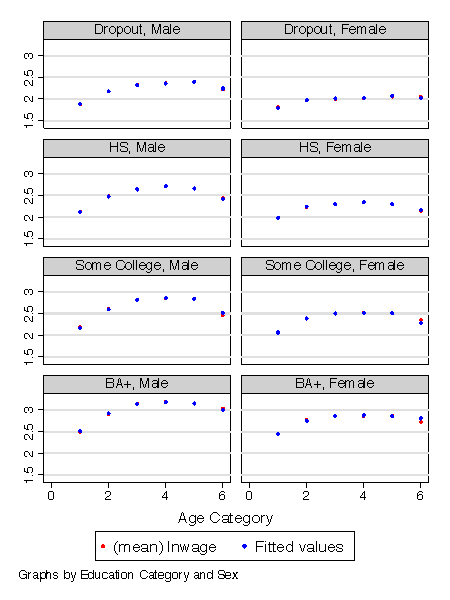
\includegraphics[scale=2]{ps2_5j.pdf}
			\end{center}
		\end{figure}

	\item A simple model which passes the chi-squared test is just lnwage on sex. We cannot reject that this model explains all of the variation in lnwage up to a sampling error.
\end{enumerate}

\newpage
\subsection*{6. Random Coefficient Binary Choice Model:}
\begin{enumerate}[a)]
	\item As was derived in the lecture notes, the simulated log likelihood can be derived as follows. Denote the Logistic cdf with $\Lambda$ and its pdf with $\lambda$.

	First observe that
	$$Pr(Y_i = 1 | X_i, b_i) = Pr(\epsilon_i > -b_i x_i) = 1- Pr(\epsilon_i < - b_i x_i) = 1- \Lambda(-b_i x_i) = \Lambda(b_ix_i)$$
	Thus, assuming that $b_i$ and $\epsilon_i$ are independent:
	$$Pr(Y_i = 1|X_i) = \int \Lambda(b x_i) \frac{1}{\sigma}\phi(\frac{b_i - \mu}{\sigma})db$$

	The likelihood of this model for a single observation is $$L(Y_i,X_i;\mu,\sigma) = \left(\int \Lambda(b x_i) \frac{1}{\sigma}\phi(\frac{b_i - \mu}{\sigma})db\right)^{Y_i}\left(1 - \int \Lambda(b x_i) \frac{1}{\sigma}\phi(\frac{b_i - \mu}{\sigma})db\right)^{1-Y_i}$$

	Thus, for \textbf{fixed} random draws $\left\{u_i\right\}_{m=1}^{M}$ from $\mathcal{N}(0,1)$, the simulated likelihood is
	$$\hat L_M(Y_i,X_i,\mu,\sigma) 
	= 
	\left(\frac{1}{M}\sum_{m=1}^M\Lambda(\underbrace{(\mu+\sigma u_{im})}_{\equiv b}X_i)\right)^{Y_i}
	\left(1-\frac{1}{M}\sum_{m=1}^M\Lambda(\underbrace{(\mu+\sigma u_{im})}_{\equiv b}X_i)\right)^{1-Y_i}
	$$
	
	Clearly, taking logs (of the product of all the likelihoods) allows us to recover the simulated log-likelihood of the full sample. 

	Let's differentiate with respect to $\mu$ and $\sigma$!

	For $\mu$:
	\begin{align*}
		\frac{\partial}{\partial \mu} & \frac{1}{N}\sum_{i}^{N} Y_i log\left(\frac{1}{M}\sum_{m=1}^M\Lambda((\mu+\sigma u_{im})X_i)\right) + (1-Y_i) log\left(1-\frac{1}{M}\sum_{m=1}^M\Lambda((\mu+\sigma u_{im})X_i)\right) \\
		= & \frac{1}{N}\sum_i^N \left[\frac{Y_iX_i\frac{1}{M}\sum_{m=1}^M\lambda((\mu+\sigma u_{im})X_i)}{\frac{1}{M}\sum_{m=1}^M\Lambda((\mu+\sigma u_{im})X_i)} - \frac{(1-Y_i)X_i\frac{1}{M}\sum_{m=1}^M\lambda((\mu+\sigma u_{im})X_i)}{1-\frac{1}{M}\sum_{m=1}^M\Lambda((\mu+\sigma u_{im})X_i)} \right] 
	\end{align*}
	For $\sigma$:
		\begin{align*}
		\frac{\partial}{\partial \sigma} & \frac{1}{N}\sum_{i}^{N} Y_i log\left(\frac{1}{M}\sum_{m=1}^M\Lambda((\mu+\sigma u_{im})X_i)\right) + (1-Y_i) log\left(1-\frac{1}{M}\sum_{m=1}^M\Lambda((\mu+\sigma u_{im})X_i)\right) \\
		= & \frac{1}{N}\sum_i^N \left[\frac{Y_i X_i\frac{1}{M}\sum_{m=1}^M\lambda((\mu+\sigma u_{im})X_i)u_{im}}{\frac{1}{M}\sum_{m=1}^M\Lambda((\mu+\sigma u_{im})X_i)} - \frac{(1-Y_i)X_i\frac{1}{M}\sum_{m=1}^M\lambda((\mu+\sigma u_{im})X_i) u_{im}}{1-\frac{1}{M}\sum_{m=1}^M\Lambda((\mu+\sigma u_{im})X_i)}\right]
		\end{align*}
	\item See \textit{max\_sml.m} file.
	\item See \textit{max\_sml.m} file.
	\item These results are invariant to initial conditions:
	$$\begin{bmatrix}\mu \\ ln(\sigma)\end{bmatrix} 
	= \begin{bmatrix} 1.6011 \\ 0.5139 \end{bmatrix}$$
	\item Let $\hat \theta_{MSL}$ denote the estimated parameters from the method of simulated likelihood and the true parameters $\theta = [\mu, \sigma]'$. Under proper specification, we know that
	$$\sqrt{N}(\hat \theta_{MSL} - \theta) \to 
	\mathcal{N}(\mathbf{0},\mathbf{H}(\theta)^{-1})$$
	By the delta-method, with $g(\theta) \equiv [\mu ln(\sigma)]'$, we have that
	$$\sqrt{N}(g(\hat \theta_{MSL}) - g(\theta)) \to 
	\mathcal{N}(\mathbf{0},\mathbf{G}\mathbf{H}(\theta)^{-1}\mathbf{G})$$
	where $$\mathbf{G} \equiv \frac{\partial g(\theta)}{\partial \theta} = \begin{bmatrix}1 & 0 \\ 0 & \frac{1}{\sigma}\end{bmatrix}$$

	When we calculate the square root of the diagonal elements of $\frac{1}{N}\mathbf{H}(\hat \theta)^{-1}$, we derive the standard errors of our estimates of $\mu$ and $\ln(\sigma)$: $(0.2633,0.3884)$.
	
	\item To calculate the standard errors for the incorrect model, we replace $\mathbf{H}(\theta)^{-1}$ with $\mathbf{H}(\theta)^{-1}\mathbf{V_s}\mathbf{H}(\theta)^{-1}$, where $\mathbf{V_s}$ is the population variance-covariance matrix of the scores---defined by the the criterion function we are maximizing. 

	Again, we use the analogy principle to replace the asymptotic variance terms with the simulated likelihood, sample averages. This yields standard errors of $\mu$ and $ln(\sigma)$: $(0.4839,0.6417)$.

\end{enumerate}

\end{document}